\باب{برقرار حالت بدلتی رو}
جبری تفاعل میں یکدم تبدیلی سے دور عارضی حالت اختیار کرتا ہے۔محدود قیمت کے وقتی مستقل کی صورت میں آخر کار عارضی دورانیہ گزر جاتا ہے اور دور ایک بار پھر برقرار حالت اختیار کر لیتا ہے۔جبری تفاعل میں یکدم تبدیلی کی غیر موجودگی میں دور برقرار صورت میں رہتا ہے۔اس باب میں ایسے ہی ادوار پر غور کیا جائے گا جن کے جبری تفاعل میں یکدم تبدیلی نہیں پائی جاتی۔ایسی صورت میں جبری حل ہی مکمل حل ہو گا۔اس باب میں مکمل حل  سے مراد جبری حل ہو گا۔ 
 
\حصہ{سائن نما تفاعل}
\اصطلاح{سائن نما}\فرہنگ{سائن نما}\حاشیہب{sinusoidal}\فرہنگ{sinusoidal} تفاعل سے مراد \اصطلاح{سائن} تفاعل \عددی{\sin \theta} اور \اصطلاح{کوسائن} تفاعل \عددی{\cos \theta} ہیں۔شکل \حوالہ{شکل_بدلتی_رو_سائن_تفاعل}-الف میں رداس \عددی{A_0} کے گول دائرے پر ایک نقطہ یکساں رفتار کے ساتھ، گھڑی کی گردش کی الٹ سمت میں، حرکت کر رہا ہے۔یہ دائرہ \اصطلاح{کارتیسی محدد}\فرہنگ{کارتیسی محدد}\حاشیہب{Cartesian coordinates}\فرہنگ{Cartesian coordinates} کے مرکز \عددی{(0,0)} پر پایا جاتا ہے۔لمحہ \عددی{t} پر زاویہ \عددی{\phase{aox}} کی قیمت \عددی{\theta} کے برابر ہے۔نقطے سے \عددی{x} محدد پر عمودی لکیر محدد کو  \عددی{x(t)}  پر ٹکراتی ہے جبکہ \عددی{y} محدد پر عمودی لکیر \عددی{y(t)} پر ٹکراتی ہے۔شکل کو دیکھتے ہوئے درج ذیل لکھا جا سکتا ہے
\begin{align}\label{مساوات_بدلتا_سائن_نما_تفاعل_الف}
y(t)&=A_0 \sin \theta
\end{align}
جہاں \عددی{A_0} موج کی چوٹی ہے جسے موج کا \اصطلاح{حیطہ}\فرہنگ{حیطہ}\حاشیہب{amplitude}\فرہنگ{amplitude} کہتے ہیں اور \عددی{\theta} کو تفاعل کا \اصطلاح{دلیل}\فرہنگ{دلیل}\حاشیہد{ایک ماہر ریاضی اپنی خیالی دنیا میں کوسائن \عددی{\cos \theta} تفاعل کے ساتھ بحث میں مصورف ہوتا ہے۔ماہر ریاضی تفاعل کو دلیل کے طور پر صفر پیش کرتا ہے۔تفاعل اس کا فوراً جواب اکائی \عددی{(\cos 0=1)} دیتا ہے۔}\حاشیہب{argument}\فرہنگ{argument} کہتے ہیں۔اس مساوات میں \عددی{\theta} از خود وقت\عددی{t} پر منحصر ہے۔

 گردش کرتا نقطہ ایک چکر میں \عددی{360^{\circ}} درجے کا زاویہ یعنی \عددی{2\pi} ریڈیئن طے کرتا ہے۔ایک چکر کاٹنے کے لئے درکار دورانیے کو \اصطلاح{دوری عرصہ}\فرہنگ{دوری عرصہ}\حاشیہب{time period}\فرہنگ{time period} کہتے ہیں جسے \عددی{T} سے ظاہر کیا جاتا ہے۔
%=========================
\ابتدا{مشق}
شکل \حوالہ{شکل_بدلتی_رو_سائن_تفاعل}-الف میں نقطہ ایک چکر \عددی{\SI{20}{\milli\second}} میں پورا کرتا ہے۔یہ نقطہ ایک سیکنڈ میں کتنے چکر پورا کرے گا۔یہ نقطہ ایک سیکنڈ میں کتنے ریڈیئن کا زاویہ طے کرتا ہے۔

جوابات:\عددی{50} چکر، \عددی{100\pi \, \si{\radian}}
\انتہا{مشق}
%========================

اگر ایک چکر کاٹنے کے لئے \عددی{T} سیکنڈ کا وقت درکار ہو تب ایک سیکنڈ میں چکروں کی تعداد  \عددی{\tfrac{1}{T}} ہو گی جسے \اصطلاح{تعدد}\فرہنگ{تعدد}\حاشیہب{frequency}\فرہنگ{frequency} کہتے اور \عددی{f} سے ظاہر کرتے ہیں۔
\begin{align}
f=\frac{1}{T}
\end{align}
تعدد کی اکائی \اصطلاح{ہرٹز}\فرہنگ{ہرٹز}\حاشیہب{Hertz}\فرہنگ{Hertz} ہے جسے \عددی{\si{\hertz}} سے ظاہر کیا جاتا ہے۔

ایک چکر \عددی{2\pi} ریڈیئن کو کہتے ہیں لہٰذا \عددی{f} چکر سے مراد \عددی{2\pi f} ریڈیئن کا زاویہ ہے۔یوں \عددی{f} تعدد پر گردش کرتا نقطہ ایک سیکنڈ میں \عددی{2\pi f} ریڈیئن کا زاویہ طے کرے گا یعنی اس کی \اصطلاح{زاویائی رفتار}\فرہنگ{زاویائی رفتار}\حاشیہب{angular speed}\فرہنگ{angular speed} کی قیمت \عددی{2\pi f} ہو گی۔زاویائی رفتار کو \عددی{\omega} سے ظاہر کیا جاتا ہے جبکہ اس کی اکائی ریڈیئن فی سیکنڈ \عددی{\si{\radian\per\second}} ہے۔
\begin{align}
\omega=2\pi f
\end{align}
زاویائی رفتار \عددی{\omega} سے گردش کرتا ہوا نقطہ \عددی{t} سیکنڈ میں \عددی{2\pi f t} ریڈیئن کا زاویہ طے کرے گا۔یوں اگر \عددی{t=0} پر نقطہ عین \عددی{x} محدد کے مثبت حصے پر ہو تب لمحہ \عددی{t} پر
\begin{align}
\theta=\omega t=2\pi f t
\end{align}
لکھا جائے گا۔یوں مساوات  \حوالہ{مساوات_بدلتا_سائن_نما_تفاعل_الف} کو
\begin{gather}
\begin{aligned}\label{مساوات_بدلتا_سائن_نما_تفاعل_ب}
y(t)&=A_0 \sin 2\pi f t\\
&=A_0\sin \frac{2\pi}{T}t\\
&=A_0 \sin \omega t
\end{aligned}
\end{gather}
لکھا جا سکتا ہے۔

برقی میدان میں \عددی{y(t)} وقت کے ساتھ بدلتے دباو یا وقت کے ساتھ بدلتی رو کو ظاہر کر سکتی ہے۔مساوات \حوالہ{مساوات_بدلتا_سائن_نما_تفاعل_ب} میں دیے تفاعل، جسے شکل \حوالہ{شکل_بدلتی_رو_سائن_تفاعل}-ب میں دکھایا گیا ہے،  کا آزاد متغیرہ وقت \عددی{t} ہے۔آپ دیکھ سکتے ہیں کہ یہ تفاعل ہر \عددی{T} سیکنڈ کے بعد اپنے آپ کو دہراتا ہے۔ اس حقیقت کو ریاضی میں درج ذیل لکھا جاتا ہے۔
\begin{align}
y(t+T)=y( t)
\end{align}
جس سے مراد یہ ہے کہ تفاعل کی قیمت لمحہ \عددی{t} اور لمحہ \عددی{t+T} پر برابر ہیں۔

\begin{figure}
\centering
\begin{subfigure}{0.5\textwidth}
\centering
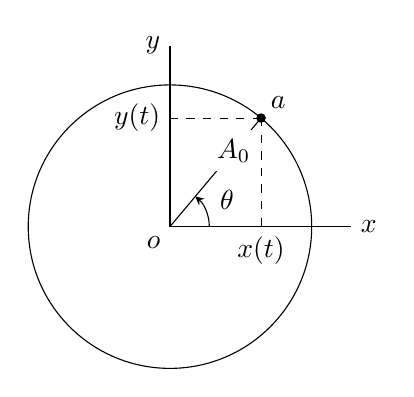
\begin{tikzpicture}
\pgfmathsetmacro{\ang}{50}
\pgfmathsetmacro{\rad}{1.8}
\pgfmathsetmacro{\xp}{\rad*cos(\ang)}
\pgfmathsetmacro{\yp}{\rad*sin(\ang)}
\draw[](0,0)--++(\rad+0.5,0)node[right]{$x$};
\draw[](0,0)--++(0,\rad+0.5)node[left]{$y$};
\draw[](0,0) circle (\rad);
\draw[fill](\ang:\rad) circle (1.5pt);
\draw(0,0)node[below left]{$o$}--++(\ang:\rad)node[pos=0.7,fill=white]{$A_0$}node[above right]{$a$};
\draw[-stealth] ([shift={(0:0.5)}]0,0) arc (0:\ang:0.5);
\draw(\ang/2:0.8)node{$\theta$};
\draw[dashed](\xp,\yp)--(\xp,0)node[below]{$x(t)$};
\draw[dashed](\xp,\yp)--(0,\yp)node[left]{$y(t)$};
\end{tikzpicture}
\caption*{الف}
\end{subfigure}
\begin{subfigure}{0.5\textwidth}
\centering
\begin{tikzpicture}
\begin{axis}[kStyleCircuitsA,small, xlabel=$t$, ylabel=$y(t)$, xtick={90,180,270,360},xticklabels={$\dfrac{T}{4}$,$\dfrac{T}{2}$,$\dfrac{3T}{2}$,$T$},ytick={-1,1},yticklabels={$-A_0$,$A_0$},
]
\addplot[domain=0:400,samples=100]{sin(x)};
\draw[gray,dashed](axis cs:0,1)--(axis cs:90,1);
\draw[gray,dashed](axis cs:0,-1)--(axis cs:270,-1);
\end{axis}%
\end{tikzpicture}%
\caption*{(ب)}
\end{subfigure}%
\begin{subfigure}{0.5\textwidth}
\centering
\begin{tikzpicture}
\begin{axis}[kStyleCircuitsA,small, xlabel=$\omega t$, ylabel=$y(\omega t)$, xtick={90,180,270,360},xticklabels={$\dfrac{\pi}{2}$,$\pi$,$\dfrac{3\pi}{2}$,$2\pi$},ytick={-1,1},yticklabels={$-A_0$,$A_0$},
]
\addplot[domain=0:400,samples=100]{sin(x)};
\draw[gray,dashed](axis cs:0,1)--(axis cs:90,1);
\draw[gray,dashed](axis cs:0,-1)--(axis cs:270,-1);
\end{axis}%
\end{tikzpicture}%
\caption*{(پ)}
\end{subfigure}%
\caption{سائن موج۔}
\label{شکل_بدلتی_رو_سائن_تفاعل}
\end{figure}%

مساوات \حوالہ{مساوات_بدلتا_سائن_نما_تفاعل_ب} کے خط کو \عددی{\omega t} کے ساتھ بھی کھینچا جا سکتا ہے۔ایسا ہی شکل \حوالہ{شکل_بدلتی_رو_سائن_تفاعل}-پ میں دکھایا گیا ہے جہاں سے واضح ہے کہ یہ تفاعل ہر \عددی{2\pi} ریڈیئن کے بعد اپنے آپ کو دہراتا ہے۔
%====================
\ابتدا{مشق}
شکل \حوالہ{شکل_بدلتی_رو_سائن_تفاعل}-الف میں گردش کرتا نقطہ \عددی{\SI{0.2}{\second}} میں \عددی{40^{\circ}} کا زاویہ طے کرتا ہے۔زاویائی رفتار، تعدد اور دوری عرصہ دریافت کریں۔

جوابات:\عددی{\omega=\tfrac{10\pi}{9}\,\si{\radian\per\second}}، \عددی{f=\SI{1.8}{\hertz}}، \عددی{T=\frac{5}{9} \, \si{\second}}
\انتہا{مشق}
%=================

شکل \حوالہ{شکل_بدلتا_لمحہ_صفر_پر_مقام_الفا_ہے} میں عمومی صورت حال دکھائی گئی ہے جہاں \عددی{\omega} زاویائی رفتار سے گردش کرتا نقطہ، لمحہ \عددی{t=0} پر  زاویہ \عددی{\alpha} پر پایا جاتا ہے۔یہ نقطہ وقت \عددی{t} کے دوران \عددی{\omega t} زاویہ طے کرتے ہوئے \عددی{\theta=\omega t+\alpha} پہنچ جائے گا لہٰذا اس کے لئے
\begin{align}\label{مساوات_بدلتا_سائن_نما_تفاعل_پ}
y(t)=A_0 \sin(\omega t +\alpha)
\end{align}
لکھا جا سکتا ہے جہاں \عددی{\alpha} کو \اصطلاح{زاویائی ہٹاو}\فرہنگ{زاویائی ہٹاو}\حاشیہب{phase angle}\فرہنگ{phase angle} کہتے ہیں۔اس مساوات کا دلیل \عددی{\omega t+\alpha} ہے۔شکل \حوالہ{شکل_بدلتا_لمحہ_صفر_پر_مقام_الفا_ہے}-ب میں مساوات \حوالہ{مساوات_بدلتا_سائن_نما_تفاعل_ب} اور مساوات \حوالہ{مساوات_بدلتا_سائن_نما_تفاعل_پ} کو دکھایا گیا ہے۔آپ دیکھ سکتے ہیں کہ ان مساوات میں \عددی{\alpha} \اصطلاح{زاویائی فرق}\فرہنگ{زاویائی فرق}\حاشیہب{phase difference}\فرہنگ{phase difference} پایا جاتا ہے۔ مساوات \حوالہ{مساوات_بدلتا_سائن_نما_تفاعل_ب} سے  مساوات \حوالہ{مساوات_بدلتا_سائن_نما_تفاعل_پ} \عددی{\alpha} ریڈیئن \اصطلاح{آگے}\فرہنگ{آگے}\حاشیہب{lead}\فرہنگ{lead} ہے۔ یہ بھی کہا جا سکتا ہے کہ مساوات \حوالہ{مساوات_بدلتا_سائن_نما_تفاعل_پ} سے مساوات \حوالہ{مساوات_بدلتا_سائن_نما_تفاعل_ب} \عددی{\alpha} ریڈیئن \اصطلاح{پیچھے}\فرہنگ{پیچھے}\حاشیہب{lag}\فرہنگ{lag} ہے۔ایک ہی تعدد کے دو تفاعل
\begin{gather}
\begin{aligned}
y_1(t)&=A_{01} \sin (\omega t +\alpha)\\
y_2(t)&=A_{02}\sin(\omega t+\beta)
\end{aligned}
\end{gather}
میں \عددی{y_1(t)} تفاعل \عددی{y_2(t)} سے  \عددی{\alpha-\beta} ریڈیئن  آگے ہے۔ہم یہ بھی کہہ سکتے ہیں کہ \عددی{y_2(t)} تفاعل \عددی{y_1(t)} سے 
 \عددی{\beta-\alpha}  ریڈیئن آگے ہے یا کہ \عددی{y_1(t)} تفاعل \عددی{y_2(t)} سے  \عددی{\beta-\alpha} ریڈیئن پیچھے ہے۔اگر \عددی{\alpha=\beta} ہو تب  تفاعل \اصطلاح{ہم زاویہ}\فرہنگ{ہم زاویہ}\حاشیہب{in phase}\فرہنگ{in phase}\فرہنگ{phase!in} کہلاتے ہیں جبکہ \عددی{\alpha\ne\beta} کی صورت میں تفاعل \اصطلاح{الگ زاویہ}\فرہنگ{الگ زاویہ}\حاشیہب{out of phase}\فرہنگ{out of phase}\فرہنگ{phase!out of} کہلاتے ہیں۔


\begin{figure}
\centering
\begin{subfigure}{0.5\textwidth}
\centering
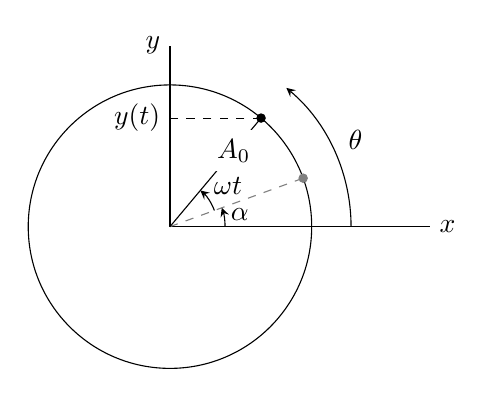
\begin{tikzpicture}
\pgfmathsetmacro{\angA}{20}
\pgfmathsetmacro{\angB}{50}
\pgfmathsetmacro{\rad}{1.8}
\pgfmathsetmacro{\xp}{\rad*cos(\angB)}
\pgfmathsetmacro{\yp}{\rad*sin(\angB)}
\draw[](0,0)--++(\rad+1.5,0)node[right]{$x$};
\draw[](0,0)--++(0,\rad+0.5)node[left]{$y$};
\draw[](0,0) circle (\rad);
\draw[gray,fill](\angA:\rad) circle (1.5pt);
\draw[fill](\angB:\rad) circle (1.5pt);
\draw[dashed,gray](0,0)--++(\angA:\rad);
\draw(0,0)--++(\angB:\rad)node[pos=0.7,fill=white]{$A_0$};
\draw[dashed](\xp,\yp)--(0,\yp)node[left]{$y(t)$};
%angles
\draw[-stealth] ([shift={(0:0.7)}]0,0) arc (0:\angA:0.7);
\draw(\angA/2:0.9)node{$\alpha$};
\draw[-stealth] ([shift={(\angA:0.6)}]0,0) arc (\angA:\angB:0.6);
\draw(\angA/2+\angB/2:0.9)node{$\omega t$};
\draw[-stealth] ([shift={(0:\rad+0.5)}]0,0) arc (0:\angB:\rad+0.5);
\draw(\angB/2:\rad+0.8)node{$\theta$};
\end{tikzpicture}
\caption*{(الف)}
\end{subfigure}%
\begin{subfigure}{0.5\textwidth}
\centering
\begin{tikzpicture}
\begin{axis}[kStyleCircuitsA,small,xlabel=$t$, ylabel=$y(t)$,ytick={1},yticklabels={$A_0$},xtick={180,360},xticklabels={$\pi$,$2\pi$},]
\addplot[domain=0:370,samples=100,dashed]{sin(x)}node[pos=0.42,pin={[font=\small]10:${A_0\sin \omega t}$},inner sep=0pt]{};
\addplot[domain=-60:320,samples=100]{sin(x+60)}node[pos=0.35,pin={[pin distance=0.75cm,font=\small]10:${A_0\sin (\omega t+\alpha)}$},inner sep=0pt]{};
\draw(axis cs:-60,-0.1)--(axis cs:-60,-0.3);
\draw[stealth-](axis cs:0,-0.2)--(axis cs:30,-0.2);
\draw[stealth-](axis cs:-60,-0.2)--(axis cs:-80,-0.2)--(axis cs:-80,-0.4)node[below]{$\alpha$};
\end{axis}
\end{tikzpicture}
\caption*{(ب) زاویائی ہٹاو۔}
\end{subfigure}%
\caption{لمحہ \عددی{t=0} پر زاویہ \عددی{\alpha} ہے۔}
\label{شکل_بدلتا_لمحہ_صفر_پر_مقام_الفا_ہے}
\end{figure}

زاویائی ہٹاو کو عموماً درجوں میں بیان کیا جاتا ہے لہٰذا \عددی{\alpha=\tfrac{\pi}{4}} کی صورت میں درج ذیل لکھا جا سکتا  ہے۔
\begin{align}\label{مساوات_بدلتا_زاویہ_ہٹاو_روایتی_طریقہ}
y(t)=A_0 \sin \left(\omega t +\frac{\pi}{4}\right)=A_0 \sin\left(\omega t+45^{\circ}\right)
\end{align}
با ضابطہ طور پر چونکہ \عددی{\omega t} کی قیمت ریڈیئن میں ہے لہٰذا \عددی{\alpha} کی قیمت بھی ریڈیئن میں ہونا لازم ہے لہٰذا تفاعل لکھنے کا صحیح طریقہ \عددی{y(t)=A_0\sin\left(\omega t+\tfrac{\pi}{4}\right)} ہی ہے لیکن زاویائی ہٹاو کو درجوں میں لکھنے کی روایت نہایت مقبول ہے لہٰذا اس کتاب میں بھی اس روایت کو برقرار رکھا جائے گا۔مساوات \حوالہ{مساوات_بدلتا_زاویہ_ہٹاو_روایتی_طریقہ} میں \عددی{45^{\circ}} لکھتے ہوئے زیر بالا میں درجے کی علامت \عددی{(^\circ)} استعمال کی گئی ہے جبکہ \عددی{\tfrac{\pi}{4}} پر کوئی علامت نہیں لگائی گئی۔اسی علامت سے ریڈیئن یا درجوں کی پہچان کی جاتی ہے۔
%================
\ابتدا{مثال}
مساوات \عددی{y_1(t)=15\sin(100t+60^{\circ})} اور \عددی{y_2(t)=22\sin(200t +0.2\pi)} کی قیمت \عددی{t=\SI{25}{\milli\second}} پر دریافت کریں۔

حل:پہلی تفاعل میں \عددی{50^{\circ}} کا زاویائی ہٹاو \عددی{\tfrac{60^{\circ}}{180^{\circ}}\times \pi=\tfrac{\pi}{3}} ریڈیئن کے برابر ہے۔یوں
 لمحہ \عددی{t=\SI{25}{\milli\second}} پر
\begin{align*}
y_1(0.025)&=15\sin\left(100\times 25\times 10^{-3}+\frac{\pi}{3}\right)=-5.918619766
\end{align*}
اور
\begin{align*}
y_2(0.025)&=22\sin(200\times 0.025+0.2\pi)=-13.39917888
\end{align*}
حاصل ہوتے ہیں۔
\انتہا{مثال}
%================== 

اگرچہ اب تک کی بحث میں ہم نے سائن تفاعل استعمال کیا، ہم اس کی جگہ کوسائن تفاعل بھی استعمال کر سکتے تھے۔ان دو تفاعل کی صورت بالکل یکساں ہے پس دونوں میں \عددی{90^{\circ}} کا زاویائی فرق پایا جاتا ہے۔
\begin{align}
\sin \left(\omega t+\frac{\pi}{2}\right)&=\cos \omega t\\
\cos \left(\omega t-\frac{\pi}{2}\right)&=\sin \omega t
\end{align}
سائن نما تفاعل کے دلیل  کے ساتھ \عددی{2\pi} ریڈیئن یا \عددی{360^{\circ}} کا مضرب جمع کرنے سے  تفاعل کی قیمت تبدیل نہیں ہوتی۔
\begin{align}
\cos(\omega t +\alpha+2\pi n)&=\cos(\omega t +\alpha) \quad \quad  n=0,\pm 1, \pm 2, \cdots \label{مساوات_بدلتا_طول_بعد_وہی_موج}\\
\sin(\omega t +\alpha+2\pi n)&=\sin(\omega t +\alpha) \quad \quad  n=0,\pm 1, \pm 2, \cdots \label{مساوات_بدلتا_طول_بعد_وہی_موج_ب}
\end{align}

دو سائن نما تفاعل میں زاویائی فرق  تین شرائط پورا کرنے کے بعد دریافت کیا جا سکتا ہے۔پہلی شرط یہ ہے کہ دونوں تفاعل کی تعدد برابر ہو۔دوسری شرط یہ ہے کہ دونوں کو  سائن تفاعل اور یا پھر دونوں کو  کوسائن تفاعل کی صورت میں لکھا جائے۔تیسری اور آخری شرط یہ ہے کہ دوسری شرط میں لکھے گئے تفاعل کے حیطے مثبت ہوں۔درج ذیل مماثل ان شرائط کو پورا کرنے میں مدد دیتے ہیں۔
\begin{align}
-\sin(\omega t+\alpha)&=\sin(\omega t+\alpha \pm 180^{\circ})\label{مساوات_بدلتا_آدھی_طول_منفی_موج_الف}\\
-\cos(\omega t+\alpha)&=\cos(\omega t+\alpha \pm 180^{\circ})\label{مساوات_بدلتا_آدھی_طول_منفی_موج_ب}
\end{align}
ان کے علاوہ درج ذیل مماثل بھی نہایت اہم ثابت ہوتے ہیں۔
\begin{align}
\sin(\alpha\pm\beta)&=\sin \alpha \cos \beta \pm \cos \alpha \sin \beta \label{مساوات_بدلتا_آدھی_طول_منفی_موج_پ}\\
\cos(\alpha \pm \beta)&=\cos \alpha \cos \beta \mp \sin \alpha \sin \beta \label{مساوات_بدلتا_آدھی_طول_منفی_موج_ت}
\end{align}
ایک آخری تفاعل جس کا ذکر ضروری ہے درج ذیل ہے۔
\begin{align} \label{مساوات_بدلتا_آدھی_طول_منفی_موج_ٹ}
\cos^2 \alpha+\sin^2 \alpha=1
\end{align}
%===============
\ابتدا{مثال}\شناخت{مثال_بدلتا_کوسائن_تفاعل_بالمقابل_ہٹاو}
درج ذیل تفاعل کے خط کھینچیں۔
\begin{itemize}
\item
$v(t)=1 \cos (\omega t +60^{\circ})$
\item
$v(t)=1 \cos (\omega t +240^{\circ})$
\item
$v(t)=1 \cos (\omega t -300^{\circ})$
\end{itemize}

حل: شکل \حوالہ{شکل_بدلتا_کوسائن_تفاعل_بالمقابل_ہٹاو}-الف میں \عددی{v(\omega t)=1\cos \omega t} کا خط دکھایا گیا ہے۔اس کو افقی محدد پر \عددی{60^{\circ}} درجے  بائیں منتقل کرنے سے \عددی{v(\omega t)=1\cos(\omega t +60^{\circ})} کا خط حاصل ہوتا ہے جسے شکل-ب میں دکھایا گیا ہے۔ ہم درج ذیل لکھ سکتے ہیں
\begin{align*}
v(\omega t)=1\cos (\omega t +240^{\circ})=1\cos (\omega t +60^{\circ}+180^{\circ})=-1\cos (\omega t +60^{\circ})
\end{align*}
جہاں مساوات \حوالہ{مساوات_بدلتا_آدھی_طول_منفی_موج_ب} کا استعمال کیا گیا ہے۔درج بالا مساوات کو شکل-پ میں دکھایا گیا ہے۔آپ دیکھ سکتے ہیں کہ یہ شکل-ب کا منفی ہے۔اسی طرح مساوات \حوالہ{مساوات_بدلتا_طول_بعد_وہی_موج} کی مدد سے
\begin{align*}
v(\omega t)=1\cos(\omega t-300^{\circ})=1\cos(\omega t-300^{\circ}+360^{\circ})=1\cos(\omega t+60^{\circ})
\end{align*}
لکھتے ہوئے شکل-ت حاصل ہوتی ہے جو عین شکل-ب ہی ہے۔
\begin{figure}
\centering
\begin{subfigure}{0.5\textwidth}
\centering
\begin{tikzpicture}
\begin{axis}[kStyleCircuitsA,small,xlabel=$\omega t$, ylabel=$v(\omega t)$,xtick={90,180,270,360}, xticklabels={$90^{\circ}$,$180^{\circ}$,$270^{\circ}$,$360^{\circ}$},ytick={-1,1},yticklabels={$-1$,$1$},]
\addplot[domain=0:360,samples=100]{1*cos(x)}node[pos=0.1,pin={[font=\small]10:${\cos \omega t}$},inner sep=0pt]{};
\end{axis}
\end{tikzpicture}
\caption*{(الف)}
\end{subfigure}%
\begin{subfigure}{0.5\textwidth}
\centering
\begin{tikzpicture}
\begin{axis}[kStyleCircuitsA,small,xlabel=$\omega t$, ylabel=$v(\omega t)$,xtick={-60,30,120,210,300}, xticklabels={$-60^{\circ}$,$30^{\circ}$,$120^{\circ}$,$210^{\circ}$,$300^{\circ}$},ytick={-1,1},yticklabels={$-1$,$1$},]
\addplot[domain=-60:300,samples=100]{1*cos(x+60)}node[pos=0.85,pin={[font=\small]170:${\cos (\omega t+60^{\circ})}$},inner sep=0pt]{};
\end{axis}
\end{tikzpicture}
\caption*{(ب)}
\end{subfigure}
\begin{subfigure}{0.5\textwidth}
\centering
\begin{tikzpicture}
\begin{axis}[kStyleCircuitsA,small,xlabel=$\omega t$, ylabel=$v(\omega t)$,xtick={-60,30,120,210,300},
 xticklabels={$-60^{\circ}$,$30^{\circ}$,$120^{\circ}$,$210^{\circ}$,$300^{\circ}$},ytick={-1,1},yticklabels={$-1$,$1$},]
\addplot[domain=-60:300,samples=100]{1*cos(x+240)}node[pos=0.85,pin={[font=\small]-170:${\cos( \omega t+240^{\circ})}$},inner sep=0pt]{};
\end{axis}
\end{tikzpicture}
\caption*{(پ)}
\end{subfigure}%
\begin{subfigure}{0.5\textwidth}
\centering
\begin{tikzpicture}
\begin{axis}[kStyleCircuitsA,small,xlabel=$\omega t$, ylabel=$v(\omega t)$,xtick={-60,30,120,210,300}, 
xticklabels={$-60^{\circ}$,$30^{\circ}$,$120^{\circ}$,$210^{\circ}$,$300^{\circ}$},ytick={-1,1},yticklabels={$-1$,$1$},]
\addplot[domain=-60:300,samples=100]{1*cos(x-300)}node[pos=0.85,pin={[font=\small]170:${\cos( \omega t-300^{\circ})}$},inner sep=0pt]{};
\end{axis}
\end{tikzpicture}
\caption*{(ت)}
\end{subfigure}%
\caption{مثال \حوالہ{مثال_بدلتا_کوسائن_تفاعل_بالمقابل_ہٹاو} کے خط۔}
\label{شکل_بدلتا_کوسائن_تفاعل_بالمقابل_ہٹاو}
\end{figure}
\انتہا{مثال}
%==========================
\ابتدا{مثال}
درج ذیل امواج کی تعدد ہرٹز میں حاصل کریں۔ امواج کے مابین زاویائی فرق دریافت کریں۔یہ بھی بتلائیں کہ کونسی موج آگے ہے۔
\begin{align*}
v_1(\omega t)&=100\sin(400t -30^{\circ})\\
v_2(\omega t)&=-250\cos(400t+0.2\pi)
\end{align*}

حل:ان امواج میں \عددی{\omega=\SI{400}{\radian\per\second}} ہے لہٰذا
\begin{align*}
f=\frac{\omega}{2\pi}=\frac{400}{2\pi}=\SI{63.66}{\hertz}
\end{align*}
ہو گا۔زاویائی فرق دریافت کرنے کی خاطر دونوں امواج کو مثبت حیطے کے کوسائن موج کی صورت میں لکھتے ہیں۔ساتھ ہی ساتھ ان کے زاویائی ہٹاو کو درجوں میں لکھتے ہیں۔یوں
\begin{align*}
v_1(\omega t)&=100\sin(400t -30^{\circ})\\
&=100\cos(400t-30^{\circ}-90^{\circ})\\
&=100\cos(400t-120^{\circ})\\
&=100\cos(400t+240^{\circ})
\end{align*}
لکھا جا سکتا ہے جہاں آخری قدم پر مساوات \حوالہ{مساوات_بدلتا_طول_بعد_وہی_موج} کا استعمال کیا گیا۔اسی طرح
\begin{align*}
v_2(\omega t)&=-250\cos(400t+0.2\pi)\\
&=250\cos(400t+0.2\pi+\pi)\\
&=250\cos(400t+216^{\circ})
\end{align*}
بھی لکھا جا سکتا ہے جہاں آخری قدم پر \عددی{1.2\pi} ریڈیئن کو \عددی{216^{\circ}} درجے لکھا گیا ہے۔ان امواج کے مابین
\begin{align*}
240^{\circ}-216^{\circ}=24^{\circ}
\end{align*}
کا زاویائی فرق پایا جاتا ہے اور موج \عددی{v_1(\omega t)} آگے ہے۔
\انتہا{مثال}
%========================
\ابتدا{مشق}
ایک دور میں درج ذیل تین رو پائے جاتے ہیں۔
\begin{align*}
i_1(1)&=30\cos(100\pi t+30^{\circ})\\
i_2(2)&=55\sin(100\pi t +40^{\circ})\\
i_3(t)&=20\sin(100 \pi t+60^{\circ})
\end{align*}
\عددی{i_2} سے \عددی{i_1} کتنی آگے ہے اور \عددی{i_3} سے \عددی{i_1} کتنی پیچھے ہے۔

جوابات:\عددی{80^{\circ}}، \عددی{-60^{\circ}} یا \عددی{300^{\circ}} 
\انتہا{مشق}
%=========================
\حصہ{سائن نما اور مخلوط جبری تفاعل}
گزشتہ باب میں دور پر مستقل جبری تفاعل مسلط  کرتے ہوئے، دور کا جبری ردعمل بھی مستقل قیمت کا حاصل ہوا۔تفرقی مساوات کا جبری ردعمل، مسلط جبری تفاعل اور اس کے تمام بلند درجی تفرق کا مجموعہ ہوتا ہے۔یوں  دور پر جبری دباو \عددی{v(t)=\sin \omega t} مسلط کرنے سے رو کا جبری ردعمل \عددی{i(t)=c_1\sin\omega t+c_2\cos\omega t} متوقع ہو گا۔پس جبری ردعمل کے مستقل \عددی{c_1} اور \عددی{c_2} معلوم کرنا باقی ہے۔
%===============
\ابتدا{مثال}\شناخت{مثال_بدلتا_مزاحمت_امالہ_جبری_حل_الف}
شکل \حوالہ{شکل_بدلتا_مزاحمت_امالہ_جبری_حل_الف} میں رو \عددی{i_j(t)} حاصل کریں۔

\begin{figure}
\centering
\begin{tikzpicture}
\draw(0,0) to [american voltage source,l={${v(t)=V_0\cos \omega t}$}]++(0,\y) to [resistor,i={$i(t)$},l={$R$}]++(\x,0) to [inductor,l={$L$}]++(0,-\y) to [short] (0,0);
\end{tikzpicture}
\caption{مثال \حوالہ{مثال_بدلتا_مزاحمت_امالہ_جبری_حل_الف} کا دور۔}
\label{شکل_بدلتا_مزاحمت_امالہ_جبری_حل_الف}
\end{figure}

حل: دور کی تفرقی مساوات لکھتے ہیں۔
\begin{align}\label{مساوات_بدلتا_مزاحمت_امالہ_جبری_حل_الف}
R i(t)+L \frac{\dif i(t)}{\dif t}=V_0 \cos \omega t
\end{align}
دور پر مسلط جبری تفاعل اور اس تفاعل کے تمام بلند درجی تفرق کا مجموعہ جبری حل کے برابر ہو گا۔
\begin{align*}
i_j(t)&=c_1 \cos \omega t+c_2\sin \omega t
\end{align*} 
اس جبری حل کو مساوات \حوالہ{مساوات_بدلتا_مزاحمت_امالہ_جبری_حل_الف} میں پُر کرتے ہوئے \عددی{c_1} اور \عددی{c_2} مستقل دریافت کرتے ہیں۔ 
\begin{align*}
R(c_1 \cos \omega t+c_2\sin \omega t)+L (-c_1 \omega \sin\omega t+c_2 \omega \cos \omega t)=V_0 \cos \omega t
\end{align*}
درج بالا مساوات میں دونوں اطراف \عددی{\cos \omega t} کے  عددی سر برابر ہوں گے۔اسی طرح دونوں اطراف \عددی{\sin \omega t} کے عددی سر برابر ہوں گے۔
\begin{align*}
c_1 R+c_2 \omega L&=V_0\\
-c_1 \omega L+c_2 R&=0
\end{align*}
ان ہمزاد مساوات کو \عددی{c_1} اور \عددی{c_2} کے لئے حل کرتے ہوئے درج ذیل ملتا ہے
\begin{align*}
c_1&=\frac{R V_0}{R^2+\omega^2 L^2}\\
c_2&=\frac{\omega L V_0}{R^2+\omega^2 L^2}
\end{align*}
لہٰذا جبری حل
\begin{align}\label{مساوات_بدلتا_جبری_حل_الف}
i_j(t)=\frac{R V_0}{R^2+\omega^2 L^2} \cos \omega t+\frac{\omega L V_0}{R^2+\omega^2 L^2} \sin \omega t
\end{align}
ہو گا۔
\انتہا{مثال}
%=================
\ابتدا{مثال}\شناخت{مثال_بدلتا_مزاحمت_امالہ_جبری_حل_ب}
درج بالا مثال میں \عددی{R=\SI{100}{\ohm}}، \عددی{L=\SI{5}{\milli\henry}}، \عددی{V_0=\SI{310}{\volt}} اور \عددی{\omega=\SI{10}{\kilo\radian\per\second}} کی صورت میں جبری حل کو مساوات \حوالہ{مساوات_بدلتا_آدھی_طول_منفی_موج_ت} کی مدد سے \عددی{i(t)=I_0\cos(\omega t-\phi)} کے طرز پر لکھیں۔

حل: مساوات \حوالہ{مساوات_بدلتا_جبری_حل_الف} میں دی گئی قیمتیں پُر کرنے
\begin{align*}
i_j(t)&=\frac{100\times 310}{100^2+(10000\times 0.005)^2} \cos \omega t+\frac{10000\times 0.005\times 310}{100^2+(10000\times 0.005)^2} \sin \omega t
\end{align*}
سے درج ذیل حاصل ہوتا ہے۔
\begin{align}\label{مساوات_بدلتا_جبری_حل_ب}
i_j(t)=2.48\cos \omega t+1.24\sin \omega t
\end{align}
مساوات \حوالہ{مساوات_بدلتا_آدھی_طول_منفی_موج_ت} سے  جبری حل کی درکار صورت کو درج ذیل لکھا جا سکتا ہے۔ 
\begin{align}\label{مساوات_بدلتا_جبری_حل_پ}
i(t)=I_0 \cos(\omega t-\phi)=I_0 \cos \phi \cos \omega t+I_0 \sin \phi \sin \omega t
\end{align}
مساوات \حوالہ{مساوات_بدلتا_جبری_حل_ب} میں \عددی{\cos \omega t} اور \عددی{\sin \omega t} کے عددی سر کو مساوات \حوالہ{مساوات_بدلتا_جبری_حل_پ} کے عددی سر کے برابر پُر کرتے ہیں۔
\begin{align}
I_0 \cos \phi &=2.48 \label{مساوات_بدلتا_جبری_حل_ت}\\
I_0 \sin \phi&=1.24 \label{مساوات_بدلتا_جبری_حل_ٹ}
\end{align}
ان ہمزاد مساوات کے مربع جمع کرتے ہوئے 
\begin{align*}
I_0^2 \cos^2 \phi+I_0^2 \sin^2 \phi=2.48^2+1.24^2
\end{align*}
ملتا ہے جس میں مساوات \حوالہ{مساوات_بدلتا_آدھی_طول_منفی_موج_ٹ} کے استعمال سے  \عددی{\cos^2 \phi+\sin^2 \phi=1} پُر کرتے ہوئے
\begin{align*}
I_0=\sqrt{2.48^2+1.24^2}=2.7727
\end{align*}
ملتا ہے۔اسی طرح مساوات \حوالہ{مساوات_بدلتا_جبری_حل_ٹ} کو مساوات \حوالہ{مساوات_بدلتا_جبری_حل_ت} سے تقسیم کرنے سے
\begin{align*}
\frac{\sin \phi}{\cos \phi}=\frac{1.24}{2.48}=\tan \phi
\end{align*}
یعنی
\begin{align*}
\phi=\tan ^{-1}\frac{1.24}{2.48}=\phase{26.6^{\circ}}
\end{align*}
ملتا ہے۔یوں جبری حل درج ذیل لکھا جائے گا
\begin{align*}
i_j(t)=2.77\cos(\omega t-26.6^{\circ})=2.77\cos(10000 t-26.6^{\circ})
\end{align*}
جہاں سے ظاہر ہے کہ دباو سے رو \عددی{26.6^{\circ}} درجے پیچھے ہے۔ 
\انتہا{مثال}
%===================
\ابتدا{مثال}\شناخت{مثال_بدلتا_مزاحمت_امالہ_جبری_حل_پ}
مثال \حوالہ{مثال_بدلتا_مزاحمت_امالہ_جبری_حل_ب} کے طرز پر مثال \حوالہ{مثال_بدلتا_مزاحمت_امالہ_جبری_حل_الف} میں حاصل کئے گئے جبری حل کو \عددی{i_j(t)=I_0\cos(\omega t -\phi)} کی صورت میں لکھیں۔

حل:مساوات \حوالہ{مساوات_بدلتا_جبری_حل_الف} میں \عددی{\cos \omega t} اور \عددی{\sin \omega t} کے عددی سر کو مساوات \حوالہ{مساوات_بدلتا_جبری_حل_پ} میں \عددی{\cos \omega t} اور \عددی{\sin \omega t} کے عددی سر کے برابر پُر کرتے ہوئے درج ذیل ملتا ہے۔
\begin{align*}
I_0 \cos \phi&=\frac{R V_0}{R^2+\omega^2 L^2}\\
I_0 \sin \phi&=\frac{\omega L V_0}{R^2+\omega^2 L^2}
\end{align*}
ان ہمزاد مساوات میں دوسری مساوات کو پہلی سے تقسیم کرتے ہوئے
\begin{align*}
\frac{\sin \phi}{\cos \phi}=\tan \phi=\frac{\omega L}{R}
\end{align*}
یعنی
\begin{align}
\phi=\tan^{-1}{\frac{\omega L}{R}}
\end{align}
ملتا ہے جبکہ دونوں ہمزاد مساوات کے مربع کا مجموعہ لیتے ہوئے
\begin{align*}
I_0^2 \cos^2 \phi+I_0^2 \sin^2 \phi=I_0^2&=\left(\frac{R V_0}{R^2+\omega^2 L^2}\right)^2+\left(\frac{\omega L V_0}{R^2+\omega^2 L^2}\right)^2 \\
&=\frac{(R^2+\omega^2 L^2)V_0^2}{(R^2+\omega^2 L^2)^2}\\
&=\frac{V_0^2}{R^2+\omega^2 L^2}
\end{align*}
یعنی
\begin{align}
I_0=\frac{V_0}{\sqrt{R^2+\omega^2 L^2}}
\end{align}
ملتا ہے۔یوں جبری حل درج ذیل لکھا جائے گا۔
\begin{align}\label{مساوات_بدلتا_جبری_حل_امالہ_مزاحمت}
i_j(t)=\frac{V_0}{\sqrt{R^2+\omega^2 L^2}} \cos \left(\omega t -\tan^{-1}{\frac{\omega L}{R}}\right)
\end{align}

\انتہا{مثال}
%========================

مساوات \حوالہ{مساوات_بدلتا_جبری_حل_امالہ_مزاحمت} سے ظاہر ہے کہ \عددی{L=0} کی صورت میں \عددی{\phi=0} ہو گا لہٰذا دباو اور رو ہم زاویہ ہوں گے جبکہ \عددی{R=0} کی صورت میں \عددی{\phi=90^{\circ}} ہو گا لہٰذا دباو سے رو \عددی{90^{\circ}} درجے پیچھے ہو گی۔مزاحمت اور امالہ کے دیگر قیمتوں کی صورت میں دباو سے رو \عددی{0^{\circ}} تا \عددی{90^{\circ}} کے مابین کسی مخصوص  درجے پر پیچھے رہے گی۔اسی لئے مزاحمت اور امالہ کے ادوار کو پیچھے رہنے والے ادوار کہا جاتا ہے۔

سلسلہ وار جڑے مزاحمت اور امالہ کے دور کا حل آپ نے دیکھا۔یقیناً اس دور کا حل سلسلہ وار جڑے دو عدد مزاحمتی دور کے حل سے کئی گنا مشکل تھا۔آپ خود تصور کر سکتے ہیں کہ زیادہ تعداد کے پرزوں کا دور حل کرنا کتنا مشکل ہو گا۔اسی مشکل کو مد نظر رکھتے ہوئے ہم \اصطلاح{مخلوط تفاعل}\فرہنگ{مخلوط تفاعل}\حاشیہب{complex function}\فرہنگ{complex function} کو پیش کرتے ہیں جس سے ادوار کا حل انتہائی آسان ثابت ہوتا ہے۔

مخلوط تفاعل اور سائن نما تفاعل کا تعلق \اصطلاح{یولر مساوات}\فرہنگ{یولر مساوات}\حاشیہب{Euler's equation}\فرہنگ{Euler's equation}
\begin{align}
e^{j\omega t}=\cos \omega t +j \sin \omega t \quad \quad \text{\RL{یولر مساوات}}
\end{align}
دیتی ہے جہاں \عددی{j=\sqrt{-1}} خیالی عدد ہے۔یولر مساوات میں \عددی{\cos \omega t} \اصطلاح{حقیقی}\فرہنگ{حقیقی}\حاشیہب{real}\فرہنگ{real} مقدار اور \عددی{\sin \omega t} \اصطلاح{خیالی}\فرہنگ{خیالی}\حاشیہب{imaginary}\فرہنگ{imaginary} مقدار ہیں۔

حقیقی دنیا میں مخلوط جبری تفاعل نہیں پایا جاتا۔اس کے باوجود، دور پر سائن نما جبری تفاعل کی جگہ مخلوط جبری تفاعل مسلط کرتے ہوئے  مخلوط حل حاصل کیا جا سکتا ہے۔مخلوط جبری تفاعل کو حقیقی جبری تفاعل اور خیالی جبری تفاعل کا مجموعہ تصور کیا جا سکتا ہے۔خطی ادوار میں مسئلہ نفاذ کے تحت تمام جبری تفاعل کی علیحدہ علیحدہ اثرات کا مجموعہ لیا جا سکتا ہے۔یوں جبری تفاعل کے حقیقی جزو سے حل کا حقیقی جزو جبکہ جبری تفاعل کے خیالی جزو سے حل کا خیالی جزو حاصل ہو گا۔یوں مخلوط حل کے خیالی جزو کو رد کرتے ہوئے حقیقی جزو کو سائن نما تفاعل کا ردعمل تسلیم کیا جاتا ہے۔اس ترکیب کو مثال کی مدد سے زیادہ آسانی سے سمجھا جا سکتا ہے۔
%====================
\ابتدا{مثال}
شکل \حوالہ{شکل_بدلتا_مزاحمت_امالہ_جبری_حل_الف} میں حقیقی جبری تفاعل \عددی{V_0\cos \omega t} کی جگہ مخلوط جبری تفاعل نسب کرتے ہوئے حقیقی \عددی{i(t)} کے لئے حل کریں۔

حل:جبری تفاعل \عددی{v(t)=V_0\cos \omega t} کی جگہ دور میں \عددی{v(t)=V_0 e^{j\omega t}} نسب کرتے ہوئے کرخوف مساوات لکھتے ہیں۔
\begin{align*}
R i(t) +L\frac{\dif i(t)}{\dif t}=V_0 e^{j \omega t}
\end{align*}
جبری تفاعل \عددی{e^{j\omega t}} کا تفرق \عددی{j\omega e^{j\omega t}} بھی جبری تفاعل ہی ہے لہٰذا درج بالا مساوات کا مخلوط حل \عددی{i_m(t)=I_0e^{j\omega t}} فرض  کرتے ہیں جہاں \عددی{I_0} نا معلوم مستقل ہے۔اس حل کو درج بالا مساوات میں پُر کرتے ہوئے
\begin{align*}
R I_0 e^{j\omega t}+L \frac{\dif}{\dif t}\left(I_0 e^{j\omega t} \right)=V_0 e^{j \omega t}
\end{align*}
درکار تفرق کے بعد
\begin{align*}
R I_0  e^{j \omega t}+j \omega L I_0e^{j\omega t}&=V_0 e^{j \omega t}
\end{align*}
ملتا ہے جس کے دونوں اطراف کو \عددی{e^{j\omega t}} سے تقسیم کرتے ہوئے درج ذیل ملتا ہے۔
\begin{align*}
R I_0+j \omega L I_0&=V_0 
\end{align*}
اس سے \عددی{I_0} حاصل کرتے ہیں۔
\begin{align*}
I_0=\frac{V_0}{R+j\omega L}
\end{align*}
یوں مخلوط رو درج ذیل لکھی جا سکتی ہے۔
\begin{align*}
i_m(t)&=I_0 e^{j\omega t}\\
&=\frac{V_0 e^{j\omega t}}{R+j\omega L}
\end{align*}
ہمیں اس کا حقیقی جزو درکار ہے۔یولر مساوات کی مدد سے درج بالا مساوات کو درج ذیل لکھا جا سکتا ہے۔
\begin{align*}
i_m(t)&=\frac{V_0 (\cos \omega t+j \sin \omega t)}{R+j\omega L}
\end{align*}
دائیں ہاتھ کسر کے بالائی اور نچلے حصے کو \عددی{R-j\omega t} سے ضرب دیتے ہیں
 \begin{align*}
i_m(t)&=\frac{V_0 (\cos \omega t+j \sin \omega t)(R-j\omega L)}{(R+j\omega L)(R-j\omega L)}\\
&=\frac{V_0(R \cos \omega t+\omega L \sin \omega t)+jV_0(R\sin \omega t-\omega L \cos \omega t)}{R^2+\omega^2 L^2}
\end{align*}
جہاں دوسرا قدم ترتیب دیتے ہوئے لکھا گیا ہے۔اس کا حقیقی جزو درکار حل ہے
\begin{align}
i(t)=\frac{V_0(R \cos \omega t+\omega L \sin \omega t)}{R^2+\omega^2 L^2}
\end{align}
جو عین مساوات \حوالہ{مساوات_بدلتا_جبری_حل_الف} ہی ہے۔
\انتہا{مثال}
%================

\حصہ{دوری سمتیہ}
